% Drawing 142/02-11 -- folder 142, batch 02, archive page 37 (PDF page 38).
% Transcription: sphère : les deux pôles, les huit sommets $R_i^{\omega}$, $P^{\omega}$, et les arcs $d_i^{\omega}$, $d_i'^{\omega}$ (méridiens, pleins ou pointillés), $a_i^{\omega}$ (petits cercles) et $b_i^{\omega}$ (le long de l'équateur). Légende : $\mathrm{VII}$.
% Kind: sphere with poles, meridians and small circles. Method 2 (schematic redraw from the facsimile). Status: partial.
% Notes: Pencil outline; the two poles, each joined by six meridians to the six vertices on the three small circles of the equator (two vertices per circle, at its left and right ends): to the left and right circles solid, to the middle (hidden) circle dashed; every meridian ends with an arrow at its vertex, and all meridians of a pole start at the same pole point. The three small circles: left (with its marked point) and right in front, each as two solid arcs between its two vertices; the middle one behind, its upper arc dashed and its lower arc solid. Along the equator: the solid arc b between the left and the right circle, the arrow from the left circle out to the left edge, and the dashed back of the equator from the left edge to the middle circle and from the middle circle to the right edge. So 2 poles and 6 vertices: the eight vertices R_i^omega, P^omega of the transcription. No labels on the figure itself (the NB and its text in the left margin are not drawn). Still differs: the arrowheads on the small circles (several, overinked) are not drawn; where the dashed back equator meets the outline is approximate. Nothing is struck. Redrawn 2026-11-09 (issue 128): to check again.
% Coordinates: 1 unit = 1 mm = 1/100 of the crop width (bbox in page fractions: [0.18, 0.46, 0.34, 0.58]).
% Redrawn by Claude (claude-opus-5-5), issue #73, 2026-11-09; not checked by a human; not compiled (no TeX in the session).
% Rights: reproduces part of the work -- behind RENDER_TRANSCRIPTS, never published by itself.
\documentclass[tikz,border=3pt]{standalone}
\usepackage{amsmath,amssymb}
\usetikzlibrary{patterns,arrows.meta}
\tikzset{pencil/.style={black!45}, struck/.style={black!35}, mark/.style={circle,draw,inner sep=1.3pt}, pt/.style={circle,fill,inner sep=0.9pt}, opt/.style={circle,draw,fill=white,inner sep=1.1pt}}
\begin{document}
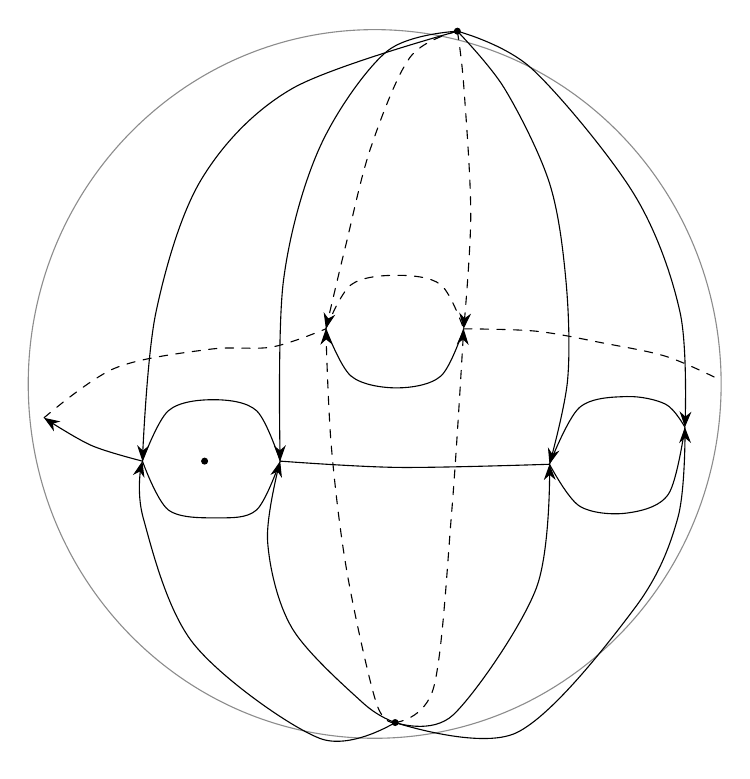
\begin{tikzpicture}[x=1mm,y=1mm,line cap=round,line join=round,font=\scriptsize]
\draw[pencil] (57,-59) ellipse[x radius=44, y radius=45];
\node[pt] at (67.5,-14.2) {};
\node[pt] at (59.6,-102) {};
\node[pt] at (35.4,-68.8) {};
\draw[-{Stealth[length=2mm]}] plot[smooth, tension=0.55] coordinates {(67.5,-14.2) (46.5,-21.5) (35,-33) (29.2,-50) (27.5,-68.8)};
\draw[-{Stealth[length=2mm]}] plot[smooth, tension=0.55] coordinates {(67.5,-14.2) (58.5,-16.8) (50,-29) (45.4,-46) (45,-68.8)};
\draw[dashed,-{Stealth[length=2mm]}] plot[smooth, tension=0.55] coordinates {(67.5,-14.2) (61.5,-17.5) (56.5,-29) (53.3,-41.5) (50.8,-52)};
\draw[dashed,-{Stealth[length=2mm]}] plot[smooth, tension=0.55] coordinates {(67.5,-14.2) (68.3,-21) (69.2,-37.5) (68.3,-52)};
\draw[-{Stealth[length=2mm]}] plot[smooth, tension=0.55] coordinates {(67.5,-14.2) (73.5,-21.5) (79.2,-33.5) (81.3,-46) (81.5,-58.5) (79.2,-69.2)};
\draw[-{Stealth[length=2mm]}] plot[smooth, tension=0.55] coordinates {(67.5,-14.2) (77,-19) (90,-35) (95.8,-50) (96.4,-64.5)};
\draw[-{Stealth[length=2mm]}] plot[smooth, tension=0.55] coordinates {(59.6,-102) (50,-104) (34,-92) (27.6,-76) (27.5,-68.8)};
\draw[-{Stealth[length=2mm]}] plot[smooth, tension=0.55] coordinates {(59.6,-102) (55.5,-99.5) (46.5,-90) (43.4,-79) (45,-68.8)};
\draw[dashed,-{Stealth[length=2mm]}] plot[smooth, tension=0.55] coordinates {(59.6,-102) (57.2,-99.5) (53.5,-83) (51.5,-67) (50.8,-52)};
\draw[dashed,-{Stealth[length=2mm]}] plot[smooth, tension=0.55] coordinates {(59.6,-102) (64.5,-97.5) (66.8,-75) (68.3,-52)};
\draw[-{Stealth[length=2mm]}] plot[smooth, tension=0.55] coordinates {(59.6,-102) (67,-101) (77.5,-85) (79.2,-69.2)};
\draw[-{Stealth[length=2mm]}] plot[smooth, tension=0.55] coordinates {(59.6,-102) (75,-103.3) (90,-87.5) (95.5,-76) (96.4,-64.5)};
\draw plot[smooth, tension=0.55] coordinates {(27.5,-68.8) (30.8,-62.4) (36.5,-61) (42,-62.4) (45,-68.8)};
\draw plot[smooth, tension=0.55] coordinates {(27.5,-68.8) (30.8,-75) (37,-76) (42,-75) (45,-68.8)};
\draw[dashed] plot[smooth, tension=0.55] coordinates {(50.8,-52) (54,-46.4) (59.8,-45.2) (65.4,-46.4) (68.3,-52)};
\draw plot[smooth, tension=0.55] coordinates {(50.8,-52) (54,-58) (59.8,-59.5) (65.4,-58) (68.3,-52)};
\draw plot[smooth, tension=0.55] coordinates {(79.2,-69.2) (83,-62) (89,-60.6) (94,-61.6) (96.4,-64.5)};
\draw plot[smooth, tension=0.55] coordinates {(79.2,-69.2) (83,-74.5) (89,-75.4) (94.3,-73) (96.4,-64.5)};
\draw plot[smooth, tension=0.55] coordinates {(45,-68.8) (60,-69.6) (79.2,-69.2)};
\draw[-{Stealth[length=2mm]}] plot[smooth, tension=0.55] coordinates {(27.5,-68.8) (21,-66.8) (15,-63.3)};
\draw[dashed] plot[smooth, tension=0.55] coordinates {(15,-63.3) (24,-57) (36,-54.6) (44,-54.3) (50.8,-52)};
\draw[dashed] plot[smooth, tension=0.55] coordinates {(68.3,-52) (77.5,-52.3) (86,-53.8) (94,-55.5) (100.5,-58.3)};
\end{tikzpicture}
\end{document}
